%\setcounter{figure}{0} % Perhaps
\renewcommand{\thefigure}{A\arabic{figure}}
\renewcommand{\thetable}{A\arabic{figure}}

\section{$\Delta$ Resonance Production and Decay Channels}
\label{appen:deltadecay}

The Clebsh-Gordon coefficients for nucleon-nucleon leading to certain $\Delta$ resonances and the respective nucleon: 
\begin{equation}
\begin{split}
& p + p \rightarrow \sqrt{\frac{3}{4}}(\Delta^{++} + n) - \sqrt{\frac{1}{4}}(\Delta^{+} + p) \\
& n + p \rightarrow \sqrt{\frac{1}{2}}(\Delta^{+} + n) - \sqrt{\frac{1}{2}}(\Delta^{0} + p)  \\
& n + n \rightarrow \sqrt{\frac{1}{4}}(\Delta^{0} + n) - \sqrt{\frac{3}{4}}(\Delta^{-} + p) 
\end{split}
\label{eq:deltaProduction}
\end{equation}

A corresponding Clebsh-Gordon coefficients for the decay of $\Delta$ pions into the constituent $\pi$ and corresponding nucleon:

\begin{equation}
\begin{split}
& p + p \rightarrow \sqrt{\frac{5}{6}}(\pi^+ + p + n) - \sqrt{\frac{1}{6}}(\pi^0 + p + p) \\
& n + p \rightarrow \sqrt{\frac{1}{6}}(\pi^+ + n + n) + \sqrt{\frac{2}{3}}(\pi^0 + n + p) + \sqrt{\frac{1}{6}}(\pi^- + p + p)  \\
& n + n \rightarrow \sqrt{\frac{1}{6}}(\pi^0 + n + n) - \sqrt{\frac{5}{6}}(\pi^- + n + p) 
\end{split}
\label{eq:pionProduction}
\end{equation}

Here we can see that that proton-proton collisions are connected with $\pi^+$ and neutron-neutron collisions are connected with $\pi^-$. 


\section{Runs analyzed in this data}

\newcommand{\hsn}{$^{132}$Sn+$^{124}$Sn}
\newcommand{\mhsn}{$^{124}$Sn+$^{112}$Sn}
\newcommand{\mlsn}{$^{112}$Sn+$^{124}$Sn}
\newcommand{\lsn}{$^{108}$Sn+$^{112}$Sn}


\begin{table}[!htb]
  \begin{center}
    \begin{tabular}{ccl}
      \hline
      System & \#runs & Run numbers \\
      \hline\hline
      \hsn & 113 & 2841, 2843, 2844, 2845, 2846, 2848, 2849, 2850, 2851, 2852, 2855, 2856, \\
      & & 2857, 2858, 2859, 2860, 2861, 2875, 2877, 2878, 2879, 2880, 2881, 2882, \\
      & & 2883, 2884, 2887, 2888, 2889, 2890, 2891, 2892, 2893, 2894, 2896, 2898, \\
      & & 2899, 2900, 2901, 2902, 2903, 2904, 2905, 2907, 2914, 2916, 2917, 2919, \\
      & & 2920, 2921, 2922, 2924, 2925, 2926, 2927, 2929, 2930, 2931, 2932, 2933, \\
      & & 2934, 2935, 2936, 2939, 2940, 2941, 2942, 2943, 2944, 2945, 2946, 2948, \\
      & & 2955, 2956, 2958, 2959, 2960, 2961, 2962, 2964, 2965, 2966, 2968, 2969, \\
      & & 2970, 2971, 2972, 2973, 2975, 2976, 2977, 2978, 2979, 2980, 2981, 2982, \\
      & & 2983, 2984, 2985, 2986, 2988, 2989, 2990, 2991, 2992, 2993, 2997, 2999, \\
      & & 3000, 3002, 3003, 3007, 3039 \\
      \hline
      \mhsn & 60 & 2542, 2543, 2544, 2546, 2547, 2548, 2552, 2553, 2554, 2555, 2556, 2557, \\
      & & 2558, 2559, 2560, 2562, 2563, 2564, 2565, 2566, 2567, 2568, 2569, 2570, \\
      & & 2571, 2572, 2573, 2574, 2575, 2578, 2579, 2580, 2581, 2582, 2583, 2584, \\
      & & 2585, 2586, 2587, 2588, 2589, 2590, 2591, 2592, 2593, 2594, 2595, 2596, \\
      & & 2597, 2598, 2599, 2600, 2601, 2617, 2618, 2619, 2620, 2621, 2622, 2623  \\
      \hline
      \mlsn & 68 & 3059, 3061, 3062, 3065, 3066, 3068, 3069, 3071, 3074, 3075, 3076, 3077, \\
      & & 3078, 3080, 3081, 3082, 3083, 3084, 3085, 3087, 3088, 3089, 3090, 3091, \\
      & & 3092, 3093, 3094, 3095, 3097, 3098, 3102, 3103, 3138, 3139, 3140, 3141, \\
      & & 3142, 3143, 3144, 3145, 3146, 3148, 3149, 3150, 3151, 3152, 3153, 3154, \\
      & & 3155, 3156, 3157, 3158, 3159, 3165, 3166, 3167, 3168, 3169, 3170, 3171, \\
      & & 3172, 3177, 3179, 3180, 3181, 3182, 3183, 3184 \\
      \hline
      \lsn & 85 & 2272, 2273, 2274, 2275, 2276, 2283, 2284, 2285, 2286, 2288, 2289, 2291, \\
      & & 2310, 2311, 2314, 2315, 2320, 2322, 2323, 2324, 2325, 2331, 2332, 2333, \\
      & & 2334, 2335, 2336, 2337, 2340, 2341, 2362, 2363, 2368, 2369, 2370, 2371, \\
      & & 2372, 2373, 2374, 2375, 2378, 2379, 2380, 2381, 2382, 2383, 2384, 2385, \\
      & & 2386, 2387, 2388, 2389, 2391, 2392, 2393, 2394, 2395, 2396, 2397, 2398, \\
      & & 2399, 2400, 2401, 2402, 2429, 2432, 2433, 2434, 2437, 2438, 2439, 2440, \\
      & & 2442, 2453, 2461, 2462, 2463, 2501, 2502, 2503, 2505, 2506, 2507, 2508, \\
      & & 2509 \\
      \hline
    \end{tabular}
    \caption{List of runs for the analysis. \label{tb:runList}}
  \end{center}
\end{table}

\clearpage

\section{Pion Yield Theory}
\label{tb:pionyieldTheory}

\begin{table*}[!htb]
\centering
\ra{1.1}
\begin{tabular}{@{}ccccccccccc@{}}
\toprule
        &  & \multicolumn{3}{c}{(a) $^{132}$Sn+$^{124}$Sn} &  & \multicolumn{3}{c}{(b) $^{108}$Sn+$^{112}$Sn} &  \\
        \cmidrule{3-5} \cmidrule{7-9} 
        Code name & $\mathrm{L~(MeV)}$ &  $\mathrm{Y}(\pi^-)$ & $\mathrm{Y}(\pi^+)$ & $\mathrm{SR}(\pi^-/\pi^+)$ &  & $\mathrm{Y}(\pi^-)$  & $\mathrm{Y}(\pi^+)$ & $\mathrm{SR}(\pi^-/\pi^+)$ &  $\mathrm{DR}(\pi^-/\pi^+)$ \\
    \midrule
        $\chi$BUU& 45.6 & 0.509 & 0.109 & 4.67 & & 0.269 & 0.134 & 2.01 & 2.33 \\
        & 120 & 0.483 & 0.117 & 4.13 &  & 0.271 & 0.140 & 1.94 & 2.13 \\
        \addlinespace[0.2cm]
        TuQMD & 54.6 & 0.779 & 0.145 & 5.37 &  & 0.442 & 0.176 & 2.51 & 2.14 \\
        & 145 & 0.839 & 0.145 & 5.79  &  & 0.474 & 0.181 & 2.62 & 2.21 \\
        \addlinespace[0.2cm]
        pBUU & 56.1 & 0.698 & 0.181 & 3.86 &  & 0.401 & 0.213 & 1.88 & 2.05 \\
        & 135 & 0.649 & 0.185 & 3.51  &   & 0.392 & 0.214 & 1.83 & 1.92 \\
        \addlinespace[0.2cm]
        AMD+JAM& 55 & 0.339 & 0.0978 & 3.47 &  & 0.200 & 0.116 & 1.72 & 2.02 \\
        & 152 & 0.311 & 0.0986 & 3.15 &  & 0.192 & 0.116 & 1.66 & 1.90 \\
        \addlinespace[0.2cm]
        IQMD-BNU & 54.6 & 0.542 & 0.148 & 3.67 &  & 0.319 & 0.175 & 1.82 & 2.01 \\
        & 145 & 0.452 & 0.153 & 2.95 &  & 0.278 & 0.167 & 1.67 & 1.77 \\
        \addlinespace[0.2cm]
        SMASH  & 55 & 0.468 & 0.168 & 2.79  &  & 0.287 & 0.190 & 1.51 & 1.85 \\
        & 152 & 0.479 & 0.163 & 2.93 &  & 0.292 & 0.188 & 1.55 & 1.89 \\
        \addlinespace[0.2cm]
        UrQMD & 46 & 0.479 & 0.129 & 3.71 &  & 0.292 & 0.144 & 2.03 & 1.83 \\
        & 104 & 0.449 & 0.133 & 3.38 &  & 0.274 & 0.147 & 1.86 & 1.81 \\
        \addlinespace[0.2cm]
        \bottomrule
    \end{tabular}
    \caption{Pion multiplicities, $Y(\pi^{\pm})$, single ratios $SR(\pi^-/\pi^+)$, and double multiplicity ratios, $DR(\pi^-/\pi^+)$ from seven transport codes. Each code uses two different symmetry energy functions, with all other parameters identical in the codes.}
    \label{tab:pionyieldTheory}
\end{table*}

\clearpage

\section{Dalitz Decay of the $\pi^0$}
\label{appen:dalitz}


\section{Cut Variation Analysis}
\label{sec:cutvar}

We employ a variety of track quality cuts described in Section~\ref{sec:qualitycut} to reduce the contamination from poorly reconstructed tracks which contribute to the background in the PID spectra. The best set of values were found for all the data sets which include the charged particle multiplicity of the event, the distance of closest approach to the vertex (DOCA), and the minimum number of clusters required for a track to be analyzed. By varying the cuts in both the data and in our MC efficiency calculations, we can evaluate the analysis to see how stable are the results with respect to these cuts. It is intuitive that while varying the cuts we will find that as the cut get tighter, and less data is included, the statistical error bar will increase. This problem is mitigated by looking at the uncorrelated error described in \cite{dataAnalysis}. Here if the systematic trend of the observable is much larger than the statistical error bars on the default cuts, with respects to the uncorrelated error bars, then there truly is some systematic trend that either exists due to physics or some error or miscalculation in the analysis. It is usually not recommended to estimated systematic error bars using this method, but sometimes it is the only way. 

Here we will discuss the particular analysis using the total pion ratio as the example. Figure~\ref{fig:totalRatioError} shows the total pion ratio as a function of several cut variations, where one cut is varied and all the others are held constant. Three cuts are of particular interest, the event multiplicity, DOCA, and the number of cluster cut.


 Figure~\ref{fig:pim_clustVar_NoEC} shows the variation as the number of clusters cut is varied before the efficiency analysis. The default cut for the number of clusters in a track is $N_c$ > 20 clusters which is represented by the middle point. The red bars represent the statistical error of this default value. The error bars on the other points are the uncorrelated error bars as described by the prescription in \cite{dataAnalysis}. Here it is clear that there is a systematic bias in the $\pi^-$ yield as we increase the number of cluster cut. This expected since cutting on the number of clusters eventually throws away short tracks that may be in the large angular regions of acceptance, thus biasing the yield. As seen in Figure~\ref{fig:pim_clustVar_EC}, this is corrected mostly be the efficiency analysis, though there seems to be some residual over correction for above 20 clusters and under correction under it, but still approximately within the statistical error bar of the default cut value of 20. 
 
When looking at the variation of the DOCA cut, we see an even better story. Before the efficiency correction in Figure~\ref{fig:pim_cutVarPOCA_NoEC}, there is very little systematic dependence, except maybe for higher values of DOCA. After efficiency correction we really see no significant variation and can safely claim there are no systematic dependencies on this particular cut. 

In Figure~\ref{fig:pim_multCutVar}, we see  a significant systematic variation of the $\pi^-$ yield as a function of the event track multiplicity. Since the event multiplicity is related to how central of a collision we had, this is purely a physics effect that is expected. This is because as the collision becomes more central, more nucleons participate in the collision due to geometric overlap. As the participating nucleons increases, there is a higher chance to make more pions, therefore the yield scales with the track multiplicity, which is ultimately related to the impact parameter as discussed in Section~\ref{sec:impact}. Therefore we should not associate any systematic error due to this effect.

There is a similar discussion that is made for the $\pi^+$ yield in the same cut variations; for the multiplicity cut in Figure~\ref{fig:pip_multCutVar}, the DOCA cut in Figure~\ref{fig:pip_cutVarPOCA}, and the cluster cut in Figure~\ref{fig:pip_clustVar}.


The analysis becomes more interesting when analyzing the total pion ratio for the same cut variation analysis performed above. Where the total pion ratio $\pi^-/\pi^+$ is plotted as a function of the multiplicity cut in Figure~\ref{fig:ratio_multCutVar}, the DOCA cut in Figure~\ref{fig:ratio_cutVarPOCA}, and the cluster cut in Figure~\ref{fig:ratio_clustVar}. Neglecting the multiplicity cut variation, which we know is derived from physical effects, it appears the pion ratio cancels out most of the systematic variations we saw previously in the single particle yields. This was expected, as the ratio tends to cancel systematic effects in the detector system. This is definitive proof of this in action. The systematic trends are less significant than the statistical error bars given in the red region for the default cuts, except maybe for a cluster cut of $N_c > 26$ which is already at the extreme end of the cut, since we know that it cuts into the particle acceptance.  



 
%show the pim total yield 
%discuss others in the apendix 


\begin{figure}[!htb]
     \centering
     \begin{subfigure}[b]{\textwidth}
         \centering
         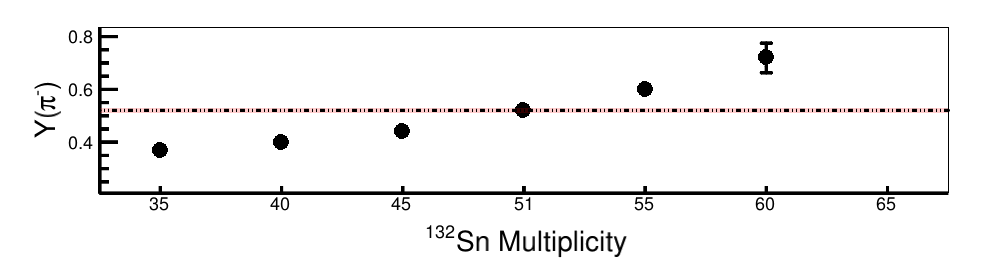
\includegraphics[width=\textwidth]{132Sn_Multiplicity_NoEC_pimTotal}
         \caption{No efficiency correction.}
         \label{fig:pim_multCutVar_NoEC}
     \end{subfigure}
     \hfill
    \begin{subfigure}[b]{\textwidth}
         \centering
         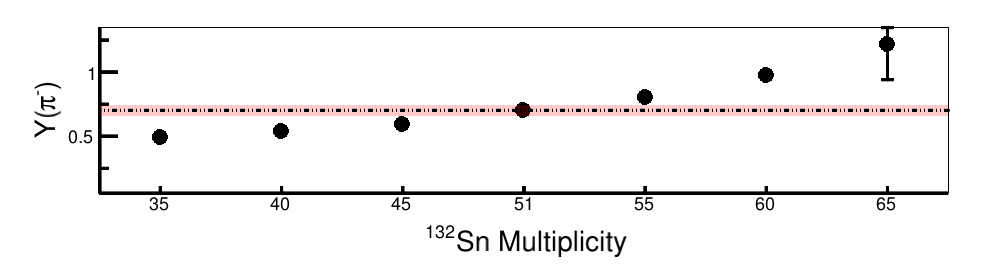
\includegraphics[width=\textwidth]{132Sn_Multiplicity_pimTotal}
         \caption{Efficiency corrected.}
         \label{fig:pim_multCutVar}
     \end{subfigure}
     \hfill
\caption{Y($\pi^-$) when varying the ${}^{132}$Sn charged particle multiplicity cut. }
\label{fig:pim_multCutVar}
\end{figure}



\begin{figure}[!htb]
     \centering
     \begin{subfigure}[b]{\textwidth}
         \centering
         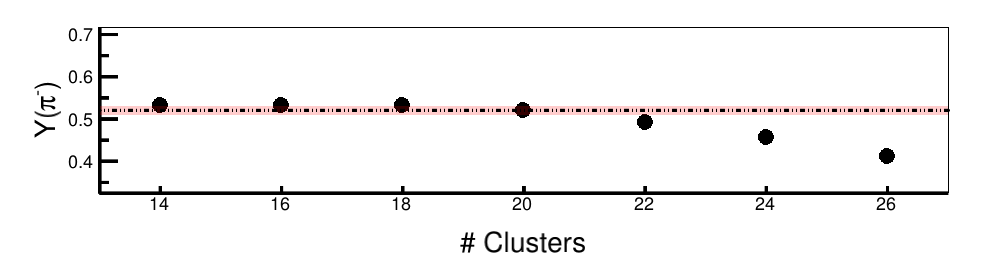
\includegraphics[width=\textwidth]{Clusters_NoEC_pimTotal}
         \caption{Before efficiency correction.}
         \label{fig:pim_clustVar_NoEC}
     \end{subfigure}
     \hfill
    \begin{subfigure}[b]{\textwidth}
         \centering
         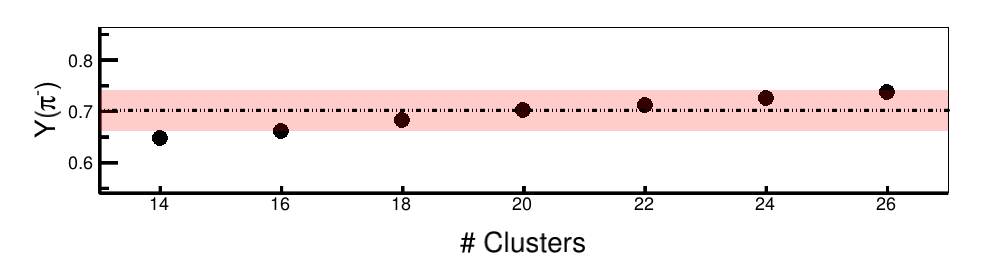
\includegraphics[width=\textwidth]{Clusters_pimTotal}
         \caption{After efficiency correction.}
         \label{fig:pim_clustVar_EC}
     \end{subfigure}
     \hfill
\caption{Y($\pi^-$) when varying the number of cluster cut of the tracks.}
\label{fig:pim_clustVar}
\end{figure}




\begin{figure}[!htb]
     \centering
     \begin{subfigure}[b]{\textwidth}
         \centering
         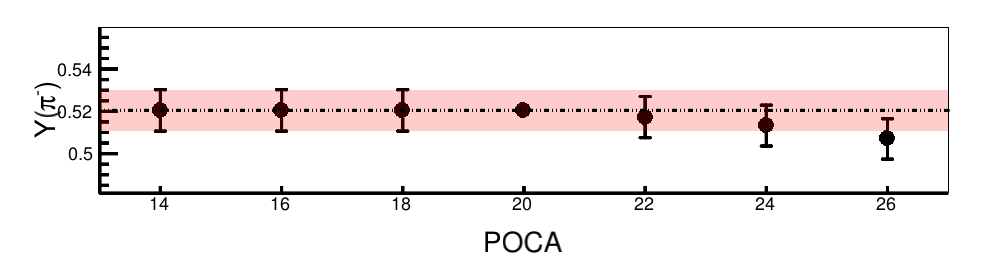
\includegraphics[width=\textwidth]{POCA_NoEC_pimTotal}
         \caption{No efficiency correction.}
         \label{fig:pim_cutVarPOCA_NoEC}
     \end{subfigure}
     \hfill
    \begin{subfigure}[b]{\textwidth}
         \centering
         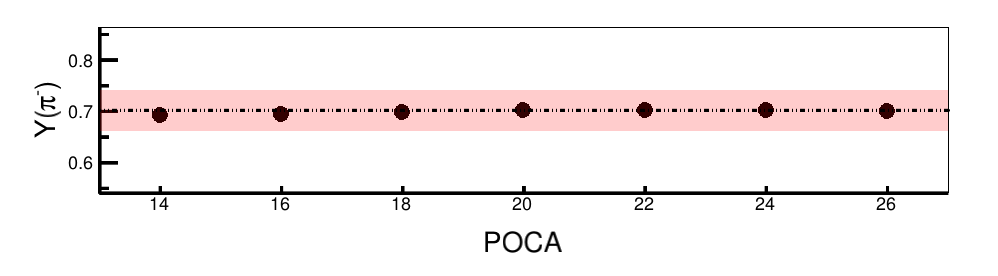
\includegraphics[width=\textwidth]{POCA_pimTotal}
         \caption{Efficiency corrected.}
         \label{fig:pim_cutVarPOCA_EC}
     \end{subfigure}
     \hfill
\caption{Y($\pi^-$) when varying the dOCA cut.}
\label{fig:pim_cutVarPOCA}
\end{figure}





\begin{figure}[!htb]
     \centering
     \begin{subfigure}[b]{\textwidth}
         \centering
         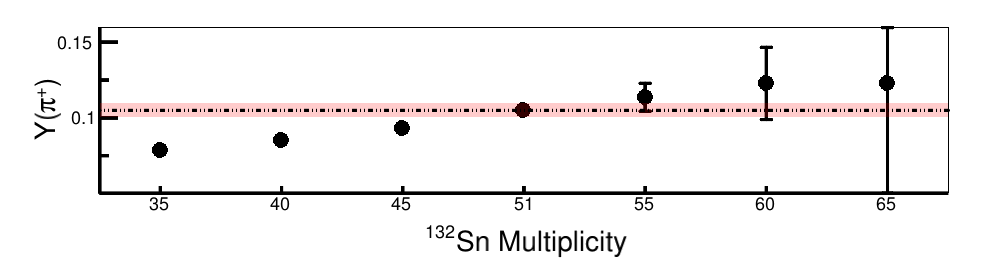
\includegraphics[width=\textwidth]{132Sn_Multiplicity_NoEC_pipTotal}
         \caption{No efficiency correction.}
         \label{fig:pip_multCutVar_NoEC}
     \end{subfigure}
     \hfill
    \begin{subfigure}[b]{\textwidth}
         \centering
         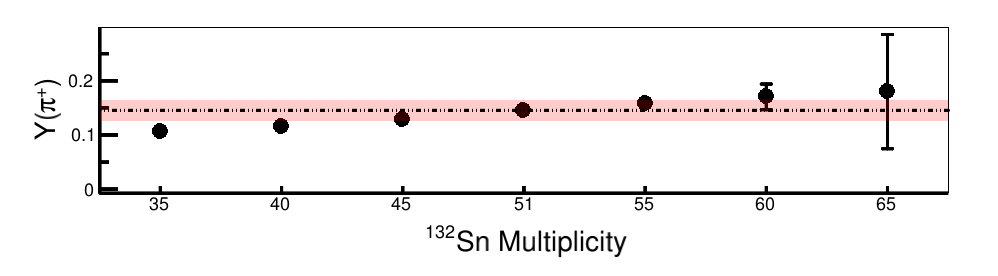
\includegraphics[width=\textwidth]{132Sn_Multiplicity_pipTotal}
         \caption{Efficiency corrected.}
         \label{fig:pip_multCutVar}
     \end{subfigure}
     \hfill
\caption{Y($\pi^+$) when varying the ${}^{132}$Sn charged particle multiplicity cut. }
\label{fig:pip_multCutVar}
\end{figure}



\begin{figure}[!htb]
     \centering
     \begin{subfigure}[b]{\textwidth}
         \centering
         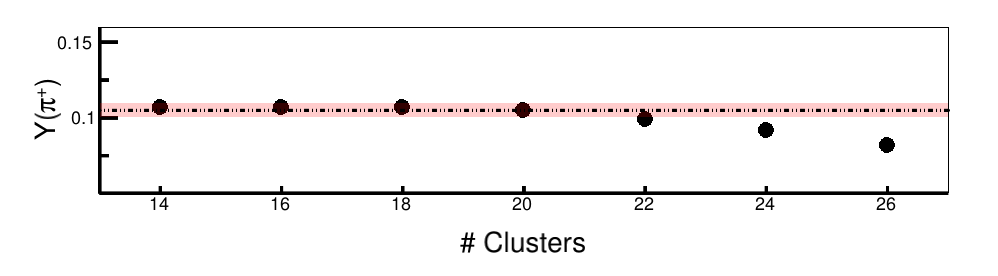
\includegraphics[width=\textwidth]{Clusters_NoEC_pipTotal}
         \caption{Before efficiency correction.}
         \label{fig:pip_clustVar_NoEC}
     \end{subfigure}
     \hfill
    \begin{subfigure}[b]{\textwidth}
         \centering
         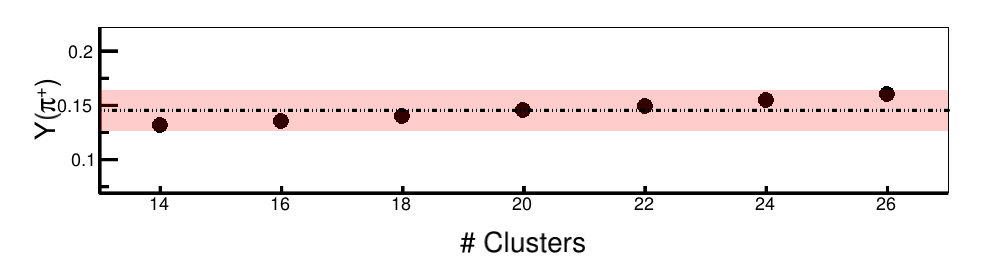
\includegraphics[width=\textwidth]{Clusters_pipTotal}
         \caption{After efficiency correction.}
         \label{fig:pip_clustVar_EC}
     \end{subfigure}
     \hfill
\caption{Y($\pi^+$) when varying the number of cluster cut of the tracks.}
\label{fig:pip_clustVar}
\end{figure}




\begin{figure}[!htb]
     \centering
     \begin{subfigure}[b]{\textwidth}
         \centering
         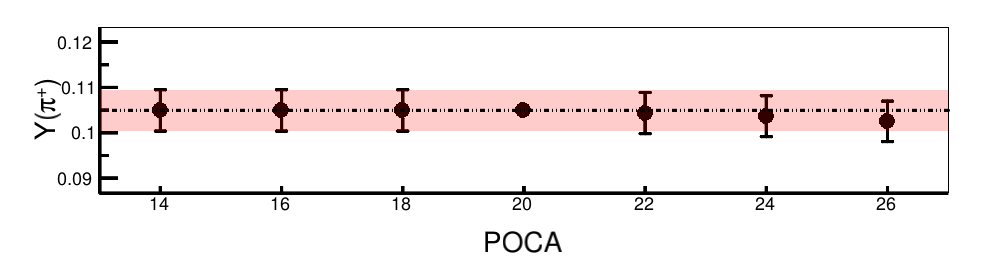
\includegraphics[width=\textwidth]{POCA_NoEC_pipTotal}
         \caption{No efficiency correction.}
         \label{fig:pip_cutVarPOCA_NoEC}
     \end{subfigure}
     \hfill
    \begin{subfigure}[b]{\textwidth}
         \centering
         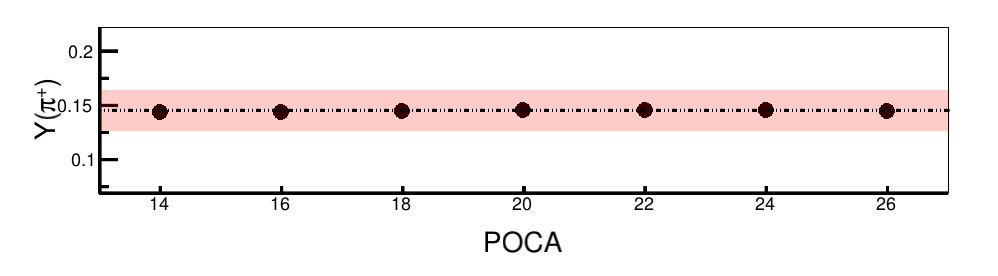
\includegraphics[width=\textwidth]{POCA_pipTotal}
         \caption{Efficiency corrected.}
         \label{fig:pip_cutVarPOCA_EC}
     \end{subfigure}
     \hfill
\caption{Y($\pi^+$) when varying the dOCA cut.}
\label{fig:pip_cutVarPOCA}
\end{figure}







\begin{figure}[!htb]
     \centering
     \begin{subfigure}[b]{\textwidth}
         \centering
         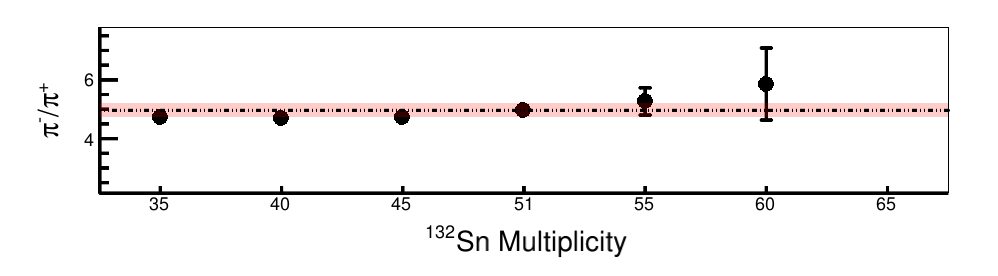
\includegraphics[width=\textwidth]{132Sn_Multiplicity_NoEC_TotalRatio}
         \caption{No efficiency correction.}
         \label{fig:ratio_multCutVar_NoEC}
     \end{subfigure}
     \hfill
    \begin{subfigure}[b]{\textwidth}
         \centering
         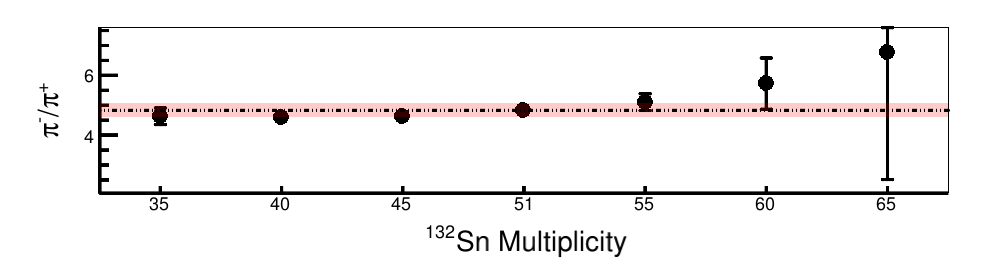
\includegraphics[width=\textwidth]{132Sn_Multiplicity_TotalRatio}
         \caption{Efficiency corrected.}
         \label{fig:ratio_multCutVar}
     \end{subfigure}
     \hfill
\caption{Y($\pi^+$)/Y($\pi^-$) when varying the ${}^{132}$Sn charged particle multiplicity cut. }
\label{fig:ratio_multCutVar}
\end{figure}



\begin{figure}[!htb]
     \centering
     \begin{subfigure}[b]{\textwidth}
         \centering
         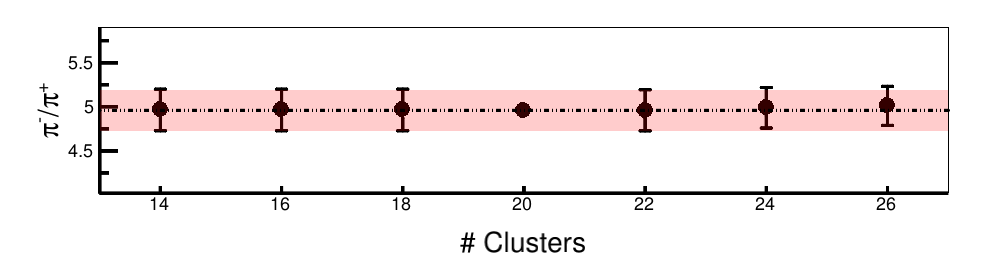
\includegraphics[width=\textwidth]{Clusters_NoEC_TotalRatio}
         \caption{Before efficiency correction.}
         \label{fig:ratio_clustVar_NoEC}
     \end{subfigure}
     \hfill
    \begin{subfigure}[b]{\textwidth}
         \centering
         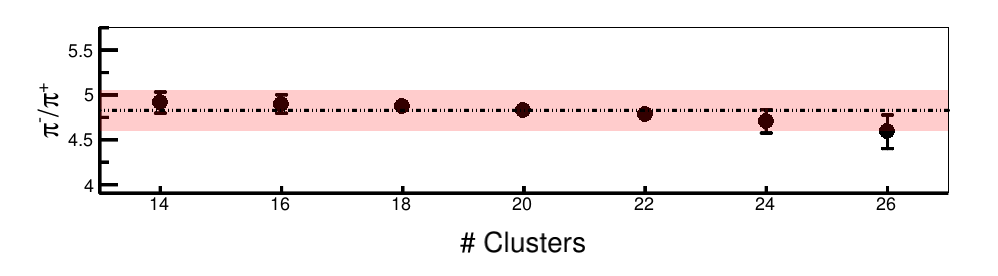
\includegraphics[width=\textwidth]{Clusters_TotalRatio}
         \caption{After efficiency correction.}
         \label{fig:ratio_clustVar_EC}
     \end{subfigure}
     \hfill
\caption{Y($\pi^+$)/Y($\pi^-$) when varying the number of cluster cut of the tracks.}
\label{fig:ratio_clustVar}
\end{figure}




\begin{figure}[!htb]
     \centering
     \begin{subfigure}[b]{\textwidth}
         \centering
         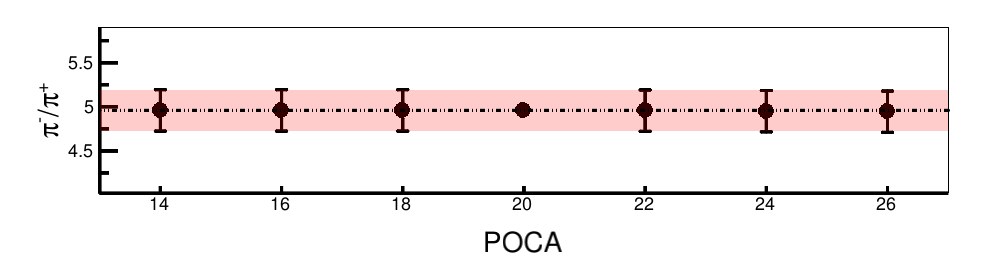
\includegraphics[width=\textwidth]{POCA_NoEC_TotalRatio}
         \caption{No efficiency correction.}
         \label{fig:ratio_cutVarPOCA_NoEC}
     \end{subfigure}
     \hfill
    \begin{subfigure}[b]{\textwidth}
         \centering
         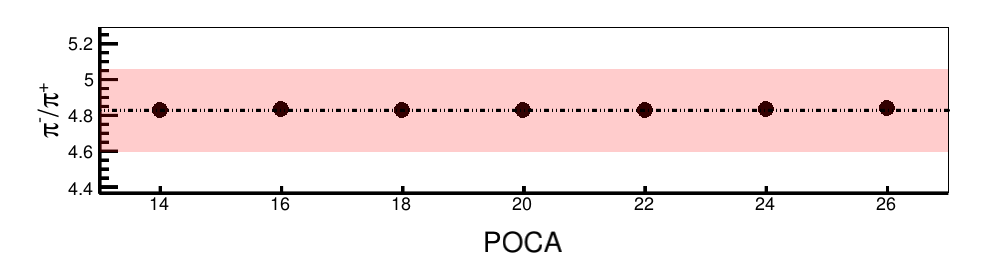
\includegraphics[width=\textwidth]{POCA_TotalRatio}
         \caption{Efficiency corrected.}
         \label{fig:ratio_cutVarPOCA_EC}
     \end{subfigure}
     \hfill
\caption{Y($\pi^+$)/Y($\pi^-$) when varying the dOCA cut.}
\label{fig:ratio_cutVarPOCA}
\end{figure}


A similar cut variation analysis was performed on the pion spectral ratio where each bin in Figure~\ref{fig:SRsn132} and \ref{fig:SRsn108} were plotted as a function of the cut parameter. Learning from the total pion ratio, we would not expect much dependence on the spectral ratio, since the ratio tends to cancel any systematic effects. Figure~\ref{fig:clusterSpectralSn132} shows the $\tin{132}{124}$ pion spectral ratio varying the number of cluster cut, after efficiency correction. Very little systematic dependence is observed except for the extreme limit of $N_c$ > 26 as was seen and discussed above. Figure~\ref{fig:docaSpectralSn132} shows the spectral ratio, varying the DOCA cut; no systematic dependence is observed. While we already know there are some physics considerations causing the multiplicity dependence I have shown the cut variation of the $\tin{132}{124}$ system multiplicity in Figure~\ref{fig:multSpectralSn132}, though no systematic error was attributed. In all no systematic errors were significant enough to add to the pion spectral ratio for the $\tin{132}{124}$ system. 




\begin{figure}[!htb]
	\centering
    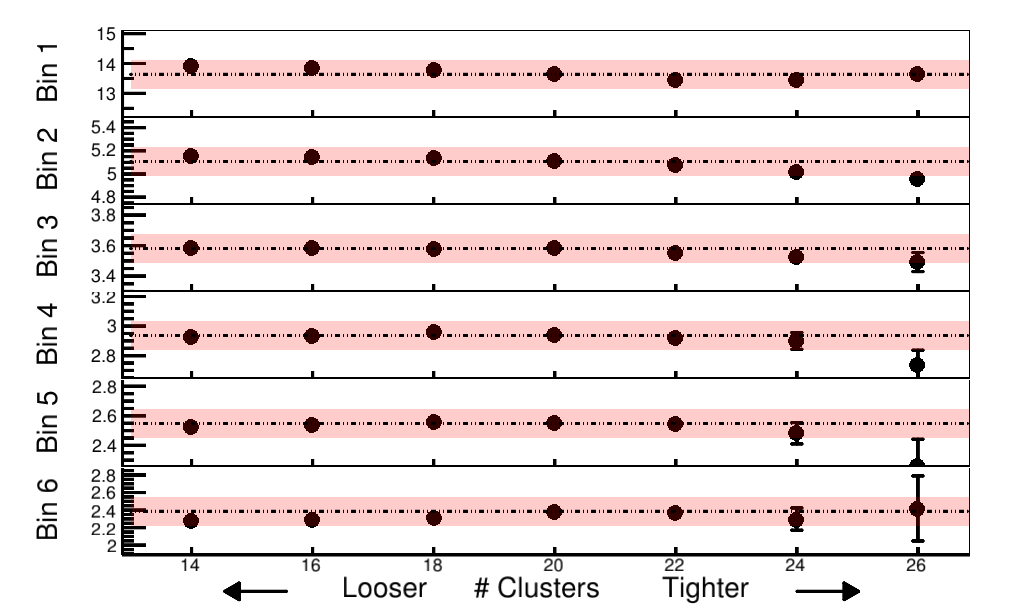
\includegraphics[width=\textwidth]{clusterSpectraSn132}
	\caption{The spectral pion ratio Y($\pi^+$)/Y($\pi^-$) when varying the cluster cut in the $\tin{132}{124}$ system.}
	\label{fig:clusterSpectralSn132}
\end{figure}


\begin{figure}[!htb]
	\centering
    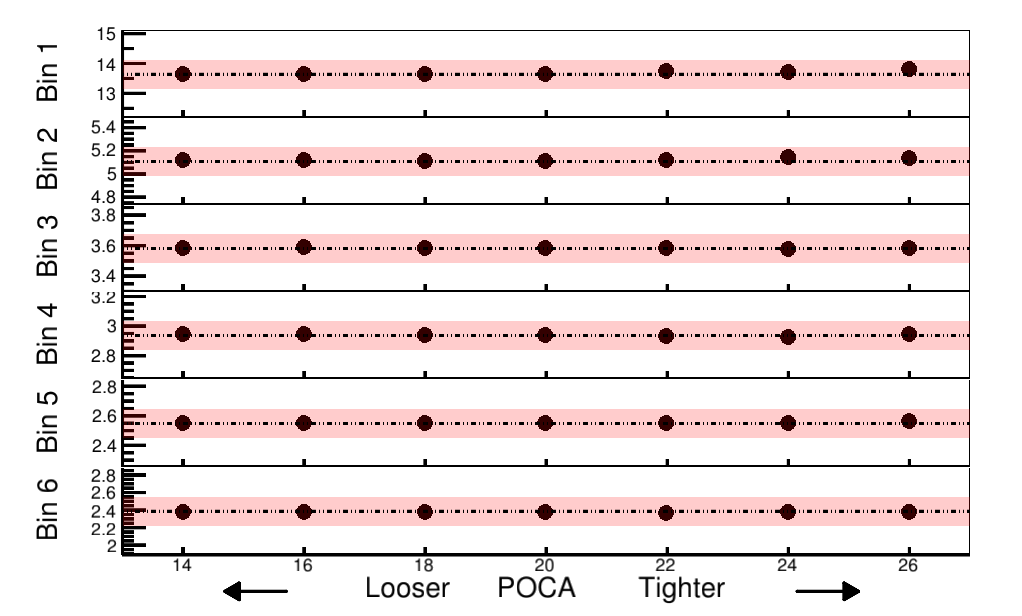
\includegraphics[width=\textwidth]{pocaSpectraSn132}
	\caption{The spectral pion ratio Y($\pi^+$)/Y($\pi^-$) when varying the DOCA cut in the $\tin{132}{124}$ system.}
	\label{fig:docaSpectralSn132}
\end{figure}


\begin{figure}[!htb]
	\centering
    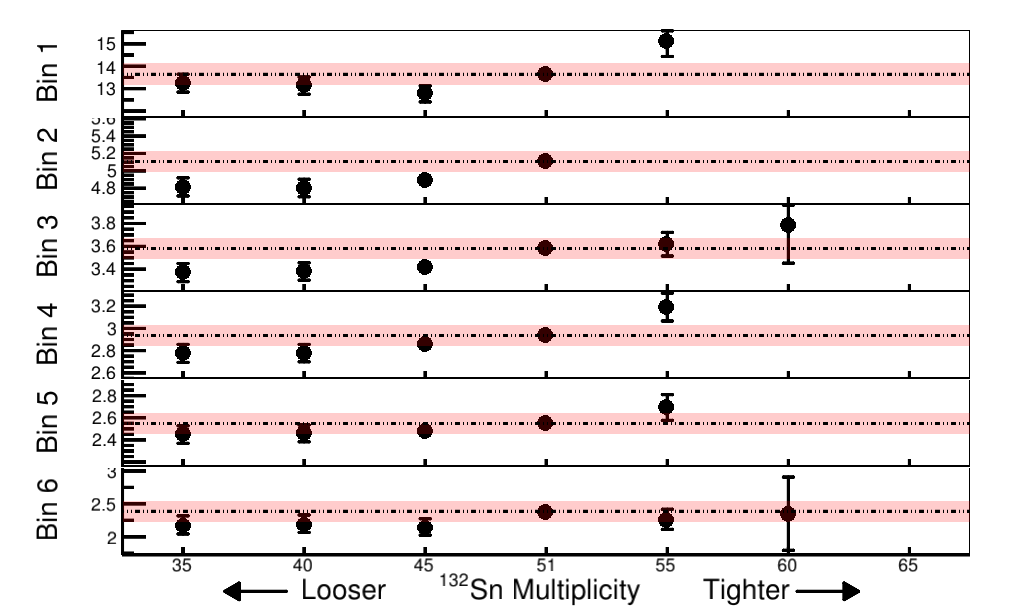
\includegraphics[width=\textwidth]{multSpectraSn132}
	\caption{The spectral pion ratio Y($\pi^+$)/Y($\pi^-$) when varying the ${}^{132}Sn$ cut.}
	\label{fig:multSpectralSn132}
\end{figure}



As we will see for the $\tin{108}{112}$ system, spectral pion ratio, the story is the exact same. Figure~\ref{fig:clusterSpectralSn108} shows the cluster cut variation, Figure~\ref{fig:docaSpectralSn108} shows the DOCA cut variation, and Figure~\ref{fig:multSpectralSn108} shows the $\tin{108}{112}$ system multiplicity cut variation.




\begin{figure}[!htb]
	\centering
    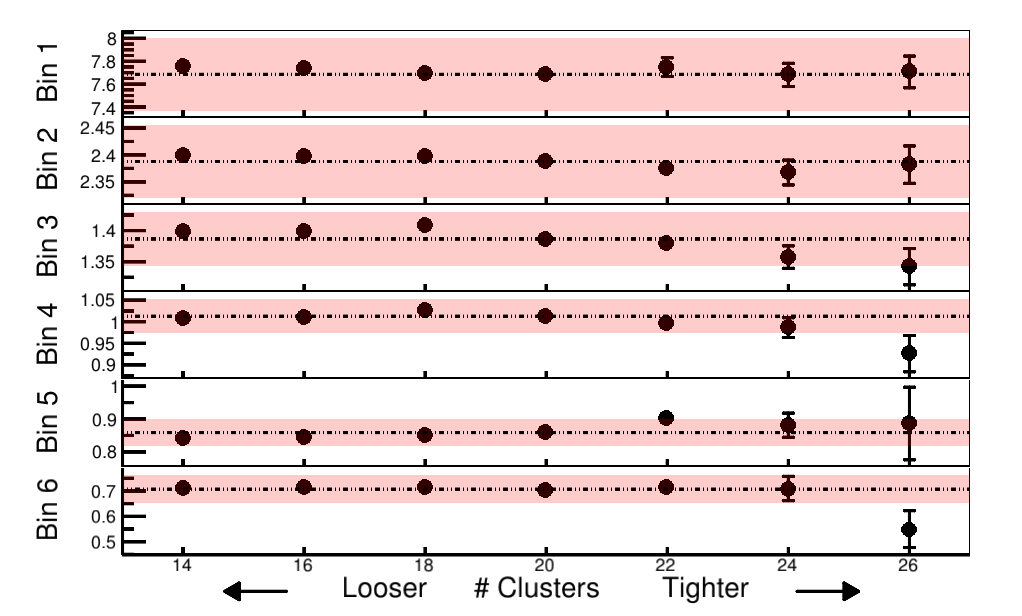
\includegraphics[width=\textwidth]{clusterSpectraSn108}
	\caption{The spectral pion ratio Y($\pi^+$)/Y($\pi^-$) when varying the cluster cut in the $\tin{108}{112}$ system.}
	\label{fig:clusterSpectralSn108}
\end{figure}


\begin{figure}[!htb]
	\centering
    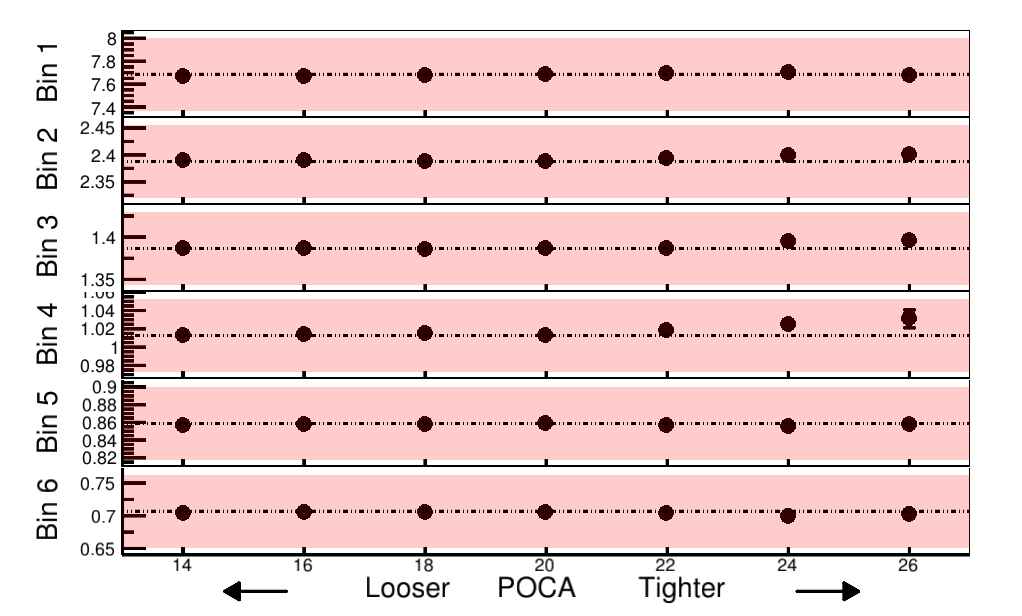
\includegraphics[width=\textwidth]{pocaSpectraSn108}
	\caption{The spectral pion ratio Y($\pi^+$)/Y($\pi^-$) when varying the DOCA cut in the $\tin{108}{112}$ system}
	\label{fig:docaSpectralSn108}
\end{figure}


\begin{figure}[!htb]
	\centering
    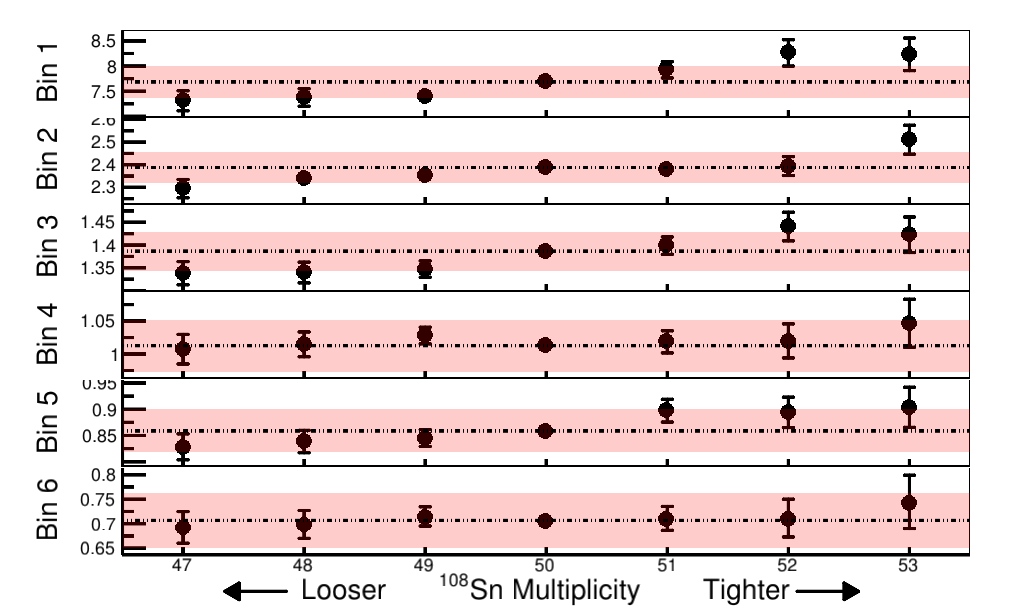
\includegraphics[width=\textwidth]{multSpectraSn108}
	\caption{The spectral pion ratio Y($\pi^+$)/Y($\pi^-$) when varying the ${}^{108}Sn$ cut.}
	\label{fig:multSpectralSn108}
\end{figure}



As with all the ratios, the double ratio also cancels systematic effects. Figure~\ref{fig:clusterDR} shows the cluster cut variation, Figure~\ref{fig:docaDR} shows the DOCA cut variation in the spectral double ratio observable. We have neglected to show the multiplicity, since we have already shown that it is derived from physics effects, and depends only on the impact parameter cut one intends to apply, not a free floating cut like the others. 



\begin{figure}[!htb]
	\centering
    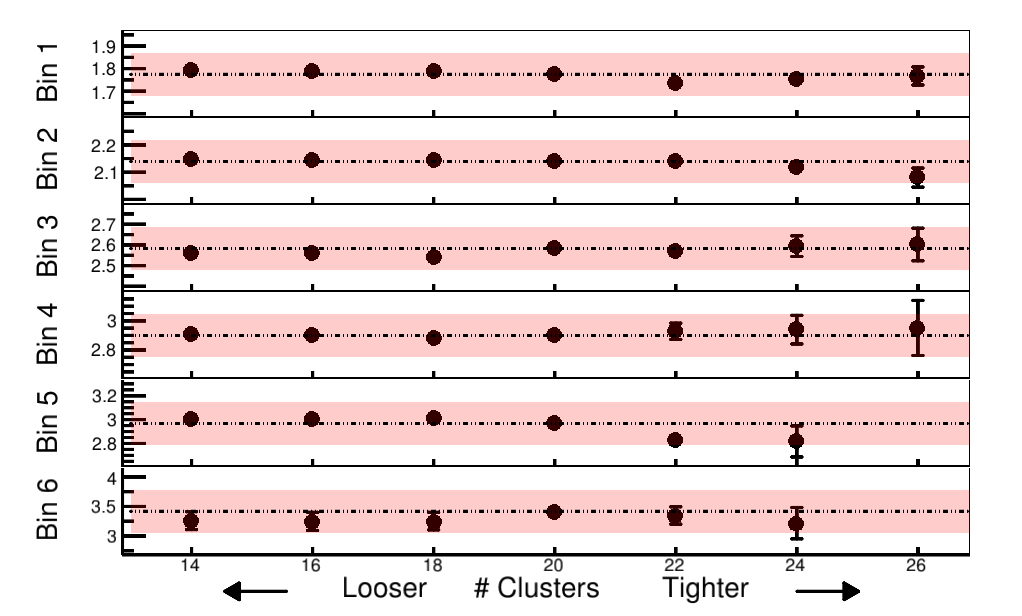
\includegraphics[width=\textwidth]{clusterDR}
	\caption{The spectral pion double ratio  when varying the cluster cut.}
	\label{fig:clusterDR}
\end{figure}


\begin{figure}[!htb]
	\centering
    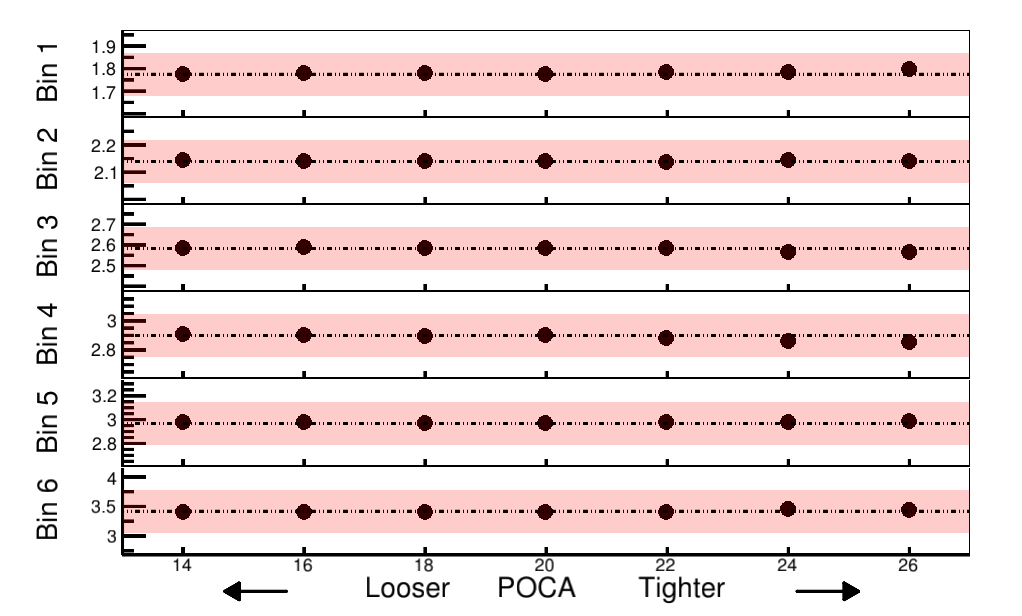
\includegraphics[width=\textwidth]{docaDR}
	\caption{The spectral pion double ratio when varying the DOCA cut.}
	\label{fig:docaDR}
\end{figure}



%\chapter{Second appendix}


